\chapter{Web Cache Object Forwarding From Desktop to Mobile for Energy Consumption Optimizations}
\addcontentsline{toc}{section}{Introduction}
\section*{Introduction}
With the beginning of the 21st century, networking support for wirelessly connected mobile user devices has fueled a continuous increase in the demand for mobile data.
Web requests now originate in a majority from wirelessly connected user devices -- a trend that Cisco, Inc. predicts to continue in the foreseeable future~\cite{VNI14}.
Simultaneously, the overall user behavior and demand for more rich media inclusion into web pages has increased the overall amount of data that is required to be transmitted per page, see, e.g., \cite{IhPa11,BuMaSe13}.
Caching on the client side has been effectively used in the past and was, together with increased numbers of parallel object downloads, able to decrease wait times for desktop clients as reported in \cite{IhPa11}.
A first view of mobile web page characteristics (which were found to exhibit lower complexity than regular desktop browser versions) and non-landing pages (which were found to be less complex than landing pages) was evaluated by the authors of~\cite{BuMaSe13}.
Moreover, a significant body of research has emerged that focuses on content delivery optimizations to mobile devices.

Typically, these optimization approaches are targeting on-device optimizations or off--device cloud--based improvements.
For mobile applications, for example, significant energy savings were found to be attainable when grouping application requests so as to avoid prolonged cellular network interface activity, see, e.g., \cite{BaBaVe09,QiWaGaHuGe12}.
Other approaches optimize the delivery to mobile devices through proxies and cloud-based data anticipation and traffic shaping, see, e.g., \cite{XiHuSaYl11}.

For web data, typically caching is used to limit the amount of data that has to be transfered to requesting clients.
In prior works focusing on mobile web page delivery optimizations, such as \cite{SaIs02}, energy optimization has been a key element, due to the limiting restrictions for mobile clients.
One particular area for optimization is the pre--fetching of web page objects combined with caching (which allows to download data before usage), such as presented in~\cite{ShKuDaWa05} with about 10 \% energy savings.
More recently, these approaches were combined with user connectivity predictions, see, e.g., \cite{ThChWo13}.

\begin{figure}
\centering
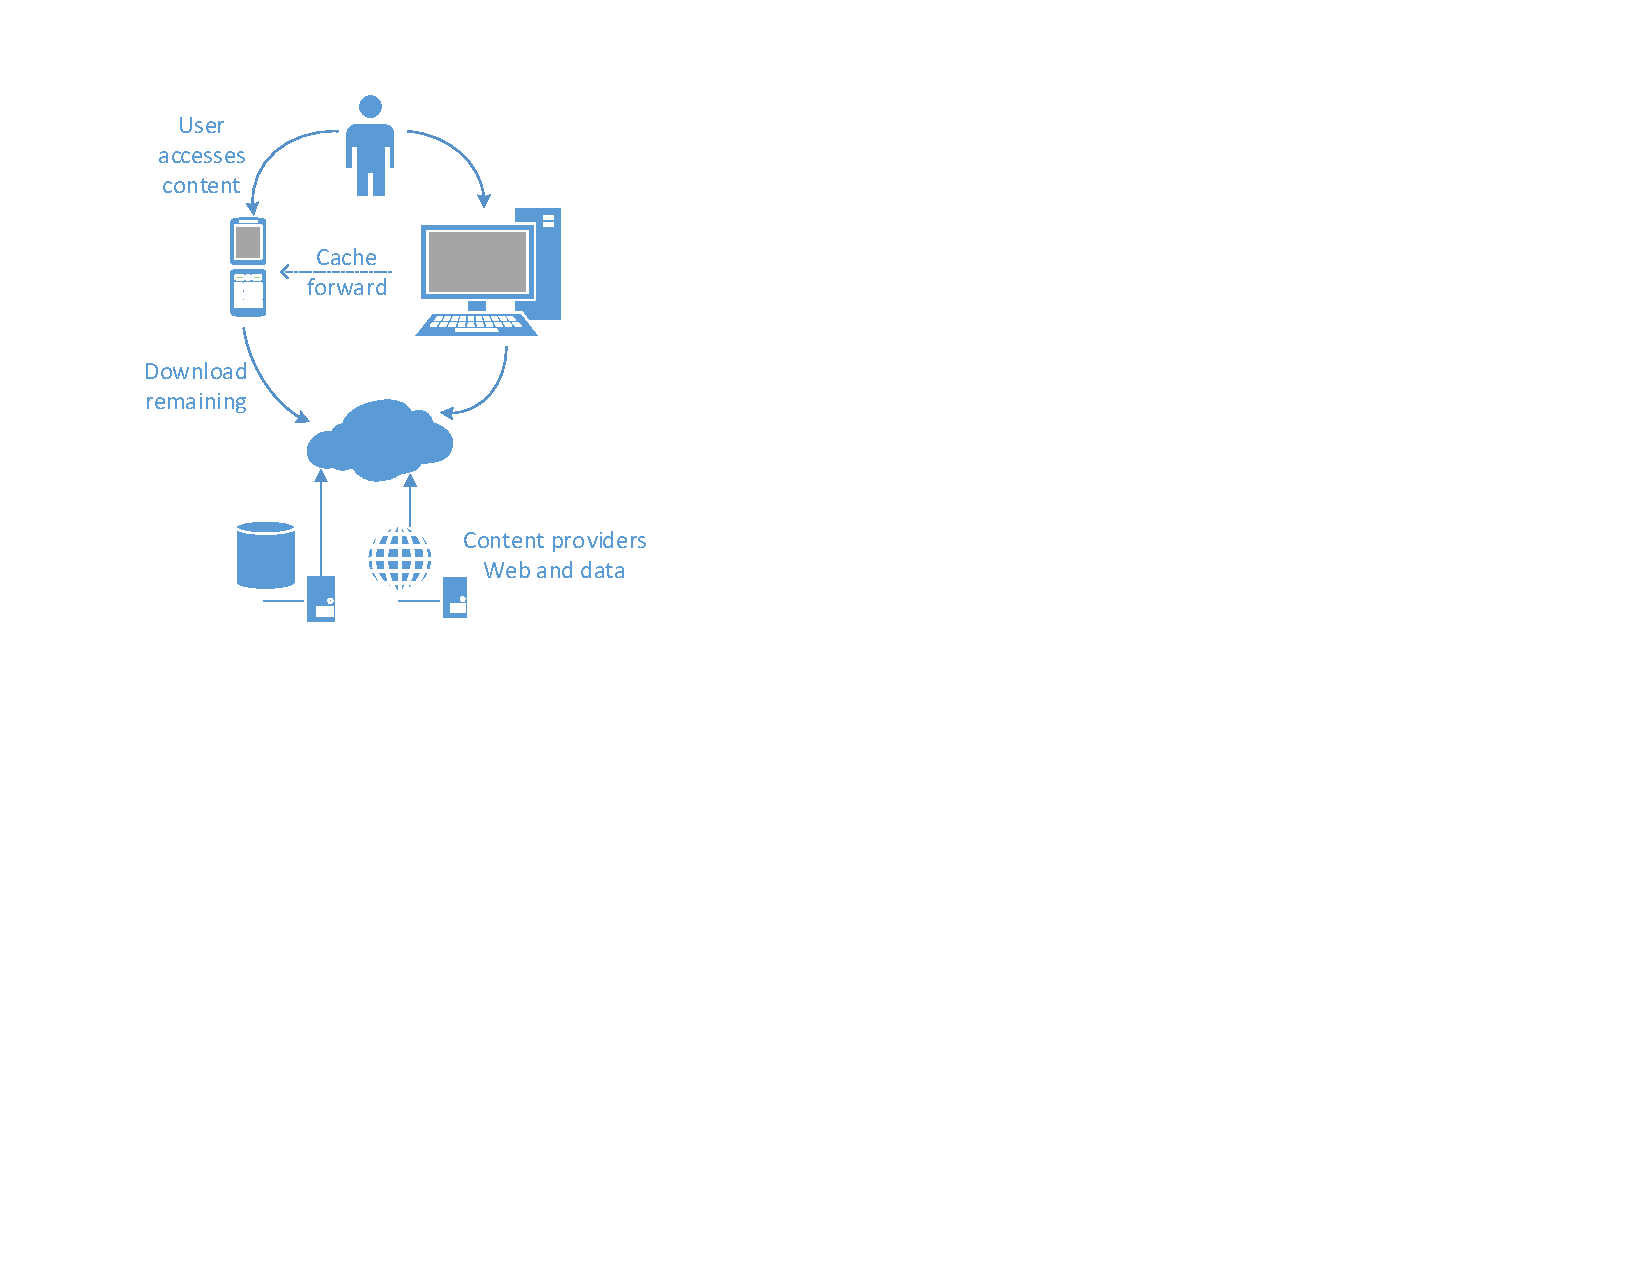
\includegraphics[scale=1,keepaspectratio]{cache_forwarding_setup}
	\caption{Screenshot of rendered web page from WebPageSpeedTest.org. As illustrated, the main textual and pictorial content items are flanked by background and interactive advertisements.}
\label{fig:cache_forwarding_setup}
\end{figure}

We propose to utilize a basic cache forwarding method that can be utilized by users to synchronize from, e.g., a desktop computer, to their mobile device, e.g., a smartphone.
We illustrate this approach in Figure~\ref{fig:cache_forwarding_setup}, which contains the desktop and a mobile device. 
As most devices are charged over night, or are at least stationary within local area network ranges, we propose to utilize this general idle period to allow direct forwarding of cached objects.
We presume that browser clients will have a shared information source in the cloud that allows the identification of visited web pages, an approach most browser clients take to date.
In turn, clients are enabled to identify web page objects that are identical between the different device display modalities, i.e., identical web objects delivered when requesting a desktop/mobile versions of a web page.
The thus transmitted objects, in turn, reside locally within the mobile device cache and do not require an energy--expensive mobile download through cellular interfaces. 
We note that the reverse of this approach is possible as well.
To support our approach, we gather data through the publicly accessible \url{WebpageSpeedTest.org} website as well as the \url{httparchive.org} archive of a large dataset of performance evaluations for popular web pages; we refer the interested reader to~\cite{Me13} for a more detailed discussion.

